%Template by Mark Jervelund - 2015 - mjerv15@student.sdu.dk

\documentclass[a4paper,10pt,titlepage]{report}

\usepackage[utf8]{inputenc}
\usepackage[T1]{fontenc}
\usepackage[english]{babel}
\usepackage{amssymb}
\usepackage{amsmath}
\usepackage{amsthm}
\usepackage{graphicx}
\usepackage{fancyhdr}
\usepackage{lastpage}
\usepackage{listings}
\usepackage{algorithm}
\usepackage{ marvosym }
\usepackage{algpseudocode}
\usepackage[document]{ragged2e}
\usepackage[margin=1in]{geometry}
\usepackage{color}
\usepackage{datenumber}
\usepackage{venndiagram}
\usepackage{chngcntr}
\usepackage[utf8]{inputenc}
\usepackage[english]{babel}
\usepackage{amssymb,amsmath,amsthm}
\usepackage{mathtools}
\newtheorem{theorem}{Theorem}

\usepackage{mathtools} % Bonus
\DeclarePairedDelimiter\norm\lVert\rVert
\setdatetoday
\addtocounter{datenumber}{0} %date for dilierry standard is today
\setdatebynumber{\thedatenumber}
\date{}
\setcounter{secnumdepth}{0}
\pagestyle{fancy}
\fancyhf{}
\title{<Course ID> <course name>}

\newcommand{\Z}{\mathbb{Z}}
\lhead{<Course id>}
\rhead{<Name> (<Student id)}
\rfoot{Page  \thepage \, of \pageref{LastPage}}
\counterwithin*{equation}{section}

\begin{document}
\begin{titlepage}
\centering
    \vspace*{9\baselineskip}
    \huge
    \bfseries
    <Title> \\
    \normalfont
    Mark Jervelund \\
    Mark@jervelund.com \\
    Doommius.com (Maybe change to m.jervelund.com or exclude ?) 	\\
    \vspace*{9\baselineskip}
    \normalfont
	\includegraphics[scale=1]{SDU_logo.png}
    \vfill\
    \vspace{5mm}
    Institute Of mathematics and Computer Science, SDU \\

	%Date
    \textbf{\datedate} \\[2\baselineskip]
\end{titlepage}

\renewcommand{\thepage}{\roman{page}}% Roman numerals for page counter
\tableofcontents
\newpage
\setcounter{page}{1}
\renewcommand{\thepage}{\arabic{page}}


\renewcommand*{\chapterpagestyle}{preamble}


  \section*{Abstract}

Databases allow modern society to store, manage and distribute data at a previously unprecedentedly scale. having data is a normal practice for most businesses, but it is often done monotonically on a single node, where modern needs require much high performance, storage, latency and  availability then current systems allow. Distributing a data store in a manner that scales performance, storage, availability and desire properties is no easy feat. In this Thesis i present methods of verifying these properties and investigate how different frameworks solve this issue, or often workaround the issue in a way that aligns with the requirements of the systems. \\

Within the framework of the thesis i present methods of verifying the ACID properties, How these properties were solved in the past, How it can and is solved today, what trade offs some systems have made, and a analysis of modern database uses cases and whether they require the ACID properties to solve issues.\\

First, I Present ACID, It's constraints, what faults occur in both database systems, how their manifests themselves, whats the underlying causes often are for these faults, and what limits the ACID properties imposes on a given system, what relaxations we can introduce to a system to still gain the same result but where we might allow conditional or future commits, eventual consistency, some degree of data-loss, dirty reads, and other relaxations in a given system.\\

Then, I Present Jepsen, a CLojure framework\cite{Jepsen} developed by K. Kingsbury that allow for testing of distributed systems, This is solved via a direct serialization graph (DSG) and queries to the target system that are carefully chosen that allows for traceability, and recoverability.  \\


Then, I present Azure Service Fabric(SF), SF is a distributed container orchestration system made my Microsoft, that allows for hosting of services, or apps. It includes a few different built in functions, but the primary interest here lie within the reliable containers aspect of SF, and what claims Microsoft makes concerning the behaviour of this data.\\

Then, I will present what modern database systems promise, what properties of ACID they follow, which they relax, and which they disregard, and well as what they gain, and which tradeoffs they endure.\\

Then i will design, and attempt to implement and execute a Jepsen test against service Fabrics reliable containers, and compare these results to the claims Microsoft has made.\\

Finally, I will present how the ACID properties compare to modern uses cases of databases, do we need to follow them strictly or can simply disregard them in some uses cases? What are the exceptions, and what is there to gain ?\\
\\



\chapter{Introduction}

Highly Distributed systems are becoming more and more common as the world grows evermore interconnected, faster paced, increasing data driven with higher expectations of services and product. where the end user expects reliability, availability combined with low- latency and cost, How do we guarantee this is a distributed system that spans the planet. Is it even possible to get both, and is it even needed in most use cases?\\

Most people are familiar with how YouTube, Facebook, Google and Reddit behave and what quirks they sometimes present, Most people remember the YouTube video counter that got stuck and only update once a day or where depending on which endpoint you connected to you were given a different numbers. These are both examples of induce eventual consistency. Here it might be that you are seeing different comments on posts depending on what region you connect from, but eventually both pages will reach consistency, 

We can also typeset \verb|<text>verbatim text</text>|.
Backticks are also rendered correctly: \verb|`words in backticks`|.





\section{ACID Properties}








\subsection{Introduction}
"
Jepsen is an effort to improve the safety of distributed databases, queues, consensus systems  (...) exploring particular systems’ failure modes. In each analysis we explore whether the system lives up to its documentation’s claims.
"\cite{jepsonio}
\\

Going from the above quite Jepsen is a way that allows us to check whether a given database system lives up to the requirements and premises that are given, and in a world where distributed, hyper scale or even planetary scale systems are becoming the norm the way data storage is done is required to behave in an expected manner, the reason that expected manner is used rather than correct manner is that we may allow certain faults to occur and eventual consistency to allow for higher throughput applications and that some data may only be required locally as to consider a transaction complete even in the case where some undesirable conditions occur, but these are tolerated to a certain extent. //

Two different examples of this is the YouTube 301 views that happened around 2015, where the number of views weren't globally distributed right away. while comments and likes were, this meant two things. //

Comments were available globally in real time, while views would also commit globally doing low load times, or off hours to maximize utilization of resources.

another more modern scenario where the real time data distribution and correctness is of the utmost importance is within transactions in the finance industry,  where we only want to consider a financial transaction committed once all shards of this data is replicated and the 'old' balance is non longer available, otherwise we could reach a condition where worst case a client is able to draw a negative balance on their account or where one of the transactions isn't recorded as only one of the two transactions is recorded.//

To go more in debt about these cases we need to do a short introduction to isolation levels and the pheomena that they can cause.


\subsection{Isolation levels and phenomena}

The Isolation level as defined by the ISO/IEC 9075 standard which defines SQL, This means that any database system should present to what level that they follow the isolation levels. in this we have 4 levels that can lead to unintended behavior within a single transaction. 

First the 3 types of behavior is explained as these are used to explain the 4 levels of isolation. the are categorized as the 3 below.
\begin{itemize}
\item dirty read,
\item Non-repeatable read and
\item Phantom read
\end{itemize}

'Dirty read' is when a S1 can read data that S2 has written but not yet committed, It is considered dirty as S2 can rollback the transaction where S1 read data that must be considered non existent. \textcolor{red}{Make example diagram} 
\\
The second case of 'Non-repeatable read' is when S1 reads data that is changed by S2 and committed. so if S1 read the some data again they will have changed. this results in two equal select statements returning different results.  \textcolor{red}{Make example diagram} 

Phantom read
The Third and last type is phantom read which is a special case of non-repeatable read that occurs when S1 reads data where a where condition is used to specify what data we want. After this initial read, a second session S2 inserts data that meets S1's where condition and commits the data. When S1 issues a select statement with the same where condition, it finds new records. It is called phantom read because the new records seem to be of phantom origin.
 \textcolor{red}{Make example diagram} 

The 4 Isolation levels are defined as:
read uncommitted
       The read uncommitted does not issue shared lock, which allows session S2 write access to the data S1 is reading.\textcolor{red}{write more in dept} 
 read commited
 \textcolor{red}{write more in dept} 
repeatable read
\textcolor{red}{write more in dept} 
serializable
\textcolor{red}{write more in dept} 



From this knowledge a table can be made that gives us an overview of the isolation levels and what behaviour and the trade off they have.
Isolation level	Read phenomena
Dirty read	Non-repeatable read	Phantom read
read uncommitted	yes	yes	yes
read committed	no	yes	yes
repeatable read	no	no	y
serializable	no	no	no
\textcolor{red}{Maybe also include something about snapshot isolation} 


\subsection{Modern Database systems, and the trade offs they make.}


Atomicity, and Isolation as we often write the data to a arbitrary node, that accepts after the data has been distributed outside of it's rack, availability zone or region. and where the newest timestamp then overrules all other written data without care of data on other nodes which can breaks Atomicity, and Isolation, as a check and set(CAS), or update statement might uses stale data and due to it's newer timestamp any data written in the meantime gets discarded. Solutions here might require waiting for full distribution of any data prior to the query executing, but this would drastically slow down the entire system. This does however not factor in issues related to system faults
"""

\subsection{Historically}

Historically this was done with using a manually defined hand coded set of patterns to check how a system behaves wrt to the isolation levels above, like if some proven invariants hold, or if an anomaly is present in parallel is present by inserting record x and y in two separate transactions and and in two more transactions checking if we can observe x but not y, or y and not x, as this could show how the systems handles long forks and snapshot isolation, and more importantly if it supports it at all.

these checking are generally quite efficient and run in polynomial time, but they only check for a certain patterns and therefor don't give us the larger picture of where issues are present, and only cover a fairly limited set of configurations and isolation levels, and are defined on a system to system basis and no interchangeability is supporter.

This means that this has been a giant scope project where case by case tests are predefined and where we only test for certain scopes, which more importantly mean that tests have been done but the test coverage haven't been perfect and a lot of anomalies are never detected.

\textcolor{red}{Need to add some more to this section, add examples are past test, diagrams, papers etc}

\subsection{State of the art.}

The State of the art is Jepsen, or rather one of the State of the Art projects.

Jepsen supports quite a few different modules but the most power full features goes by the name Elle, inferring isolation anomalies from Experimental Observations. \\

The way this works is be inferring a dependency graph between client side observations and the database version history. This is done by carefully selecting database objects and operations such that the database reads reveals information about the version history. 

this means that Elle is able to reveal any anomaly and provide a concise explanation as to why a fault occurred with information of what conditions were present to cause this fault to occur. Using this information we are able to say how a system behaves, what level of isolation and which behavior we'll see as well as what promises the system makes and how does promises are reflected in reality.

And these things can be manifested in multiple ways, some cases are as mentioned earlier in the paper accepted as eventually consistency and performance is valued higher or some applications where loosing some data points are acceptable to allow for higher write throughput.

and the same does for stale, dirty, non-repeatable and phantom reads aren't an issue. this could be on hyper scale social networks where if you see something that was deleted, or if the newest posts, comments and likes aren't distributed across the all notes, but they will eventually. but this is a trade off that is done to allow for much higher write performance as the chance a user is making chancing to the same page on two different nodes/clusters are minimal and the required performance drop required to facilitate the guarantee that all data is always up to date would mean that the system wouldn't scale at the rate it's required, this also brings up another interesting topic, approximate programming, where a program doesn't always have to return the correct output, but if we can see a magnitude speedup of a program and accept a faulty result rate of a few \%, then the cost saving and capacity increase could very much be worth it. this could be in the case of Netflix and amazon recommencing products and services, it doesn't have to be perfect and maybe sometimes the result is wrong but if it means we're able to serve a lot more customers before having to degrade services or maybe having it as a step in the service degradation levels to support as many users as possible. \\

but a lot of this lay outside the scope of this thesis but it's also a super interesting field that will probably see grow in the next decade.





\subsection{Past jepsen tests}

https://aphyr.com/posts/294-call-me-maybe-cassandra


https://aphyr.com/posts/291-call-me-maybe-zookeeper







\subsection{methods used in Jepsen tests}

\subsection{related work to Jepsen}


K. Kingsbury. Knossos.
https://github.com/jepsen-io/knossos, 2013-2019.

G. Lowe. Testing and Verifying Concurrent Objects.
Concurrency and Computation: Practice and
Experience, 29(4), 2017

J. M. Wing and C. Gong. Testing and Verifying
Concurrent Objects. Journal of Parallel and
Distributed Computing, 17(1-2), 1993.

P. B. Gibbons and E. Korach. Testing shared
memories. SIAM Journal on Computing, 26(4), 1997

S. Burckhardt, C. Dern, M. Musuvathi, and R. Tan.
Line-up: A Complete and Automatic Linearizability
Checker. PLDI ’10, 2010.


\section{Service Fabric}

\subsection{Introduction}

Service Fabric (SF) is a presented as a distributed systems platform something akin to Kubernetes (K8S), where the user is able to build, deploy and scale micro services and containers, one of the key points presented by on Azure Service Fabric is that you're able to run stateful services. It's presented by Microsoft as the backbone of their core services and data stores.


\subsection{DataStore}

So as mentioned above Service Fabric Contains stateful services, these use reliable collections that are in memory storage 



\subsection{Promises}


\subsection{Configuration}


What we are able to tweak


\subsection{What aspects of the service fabric are we  we'd like to test}

Reliable collections.

\subsection{What does service Fabric promise wrt ACID}

https://docs.microsoft.com/en-us/azure/service-fabric/service-fabric-reliable-services-reliable-collections-transactions-locks


\section{Experiment}

\subsection{Designing the experiment}

\subsection{Development}

\subsection{Issues}

Linux and windows versions being far from interchangeable and applications and services that function on windows/local machines fail crash on deployed cluster

visual studio being unable to load .dmp files to debug crashed applications from the cloud.

Visual studio remote debugger not working

\subsubsec{Azuer}

Configuration issues,

Cluster cecoming unhealty/corrupt and nodes not being configred correctly after a reimage.

\subsection{Introduction}

The Goal of the experiment to to investigate weather Service Fabric is compliance with ACID or not,


\subsection{Tooling}


%LaTeX hints are provided in \cref{chap:latexhints}.

%\blinddocument

\chapter{Related Work}

\chapter{Conclusion and Outlook}
\section*{Conclusion}

\section*{Outlook}

\printbibliography

All links were last followed on March 17, 2018.



\newpage
\appendix
\section{'Jepsen methods usage for ACID compliance in Hyperscale Cloud Frameworks'}

\section{Introduction}
The goal of this project is to assess how Jepsen\footnote[1]{https://aphyr.com/tags/jepsen } tests allow us to verify the properties of ACID\footnote[2]{Database Management Systems by Raghu Ramakrishnan \& Johannes Gehrke  ISBN13 9780071231510} in a cloud system.
The Jepsen test is a method used to evaluate the compliance of a system in relation to the ACID properties. This is done is by analysing the system via Blackbox\footnote[3]{https://youtu.be/tRc0O9VgzB0?t=293} tests , in the sense that the internals of the system work are not relevant. We look at the service from a client-side and not any underlying structures or frameworks.
The ACID properties are 
\begin{itemize}
\item	Atomicity \\
Guarantees that each transaction is treated as a single "unit", which either succeeds completely or fails completely 
\item	Consistency \\
Ensures that a transaction can only bring the database from one valid state to another
\item	Isolation \\
Ensures that concurrent execution of transactions leaves the database in the same state that would have been obtained if the transactions were executed sequentially 
\item	Durability \\
Guarantees that once a transaction has been committed, it will remain committed even in the case of a system failure 
\end{itemize}
\footnote[2]{Database Management Systems by Raghu Ramakrishnan \& Johannes Gehrke  ISBN13 9780071231510} \\
We plan to apply these methods on Service Fabric\footnote[4]{https://docs.microsoft.com/en-us/azure/service-fabric/service-fabric-overview  } , to verify if this system is compliant with the ACID properties. Service Fabric is a framework developed by Microsoft, designed to allow developers to build Hyper-Scale Cloud (HSC) deployments on the Azure\footnote[5]{https://microsoft.com/en-us/azure/ } platform.
The motivation behind this thesis is to study the ACID properties in an HSC environment and evaluate how the constraints of ACID hold up in practice, as well as verifying if these constraints are met, and more importantly if they are not. 
\section{Plan}
     
The project is segmented into three parts. The writing of the report will take place at all times throughout the process, and the final phase should be a finalization and corrections phase.  
\subsection{The study phase  }
\begin{itemize}
\item	The first part of the study will focus on analysing the previous\footnote[6]{https://jepsen.io/analyses } Jepsen tests performed on other systems. This will allow us to define a strategy in terms of: which tools, tactics and methods are worth investigating, and what type of faults should be taken note of. This information is useful for two aspects:
\begin{itemize}
\item	where our focus should be when testing,  
\item	which tools and packages we should be familiarize with. 
\end{itemize}
\item	 The second part of the study will centre around “Service Fabric” and getting to know how the framework is coupled together, what vectors we can access the system from, and how we can manipulate the framework to induce fault conditions.   
\end{itemize}
\subsection{The experimentation phase}
\begin{itemize}
\item	In the experimentation phase, we will design and perform tests on the system. If any faults occur, we will attempt to locate where, and why they occur. If the scope and the timeline of the project allow, we will assess whether we prevent the faults from occurring in the future.
\item	The Experimentation phase of the project will include the steps described below. 
\begin{itemize}
\item	Planning of the test, selection of the aspects of the system to be tested, consulting with developers and users of the system to determine if and where undesired behaviour may occur.
\item	Designing the tests and setting up the tools to facilitate those tests.
\item	Writing the tests, verifying they work as intended and setting up a data collection framework to collect the data in a manner that allows our analysis.
\item	Performing the tests on the system in different scenarios, normal conditions and different levels of faults and disaster recovery.
\item	Analysing the data for faults, errors and inconsistencies.
\item	Consulting with DEVs to determine where the faults occurred, and which failures or bugs led to these fault conditions.
\item	Concluding whether “Service Fabric” is ACID-compliant. 
\end{itemize}
\end{itemize}
\subsection{The report phase }
\begin{itemize}
\item The final phase of the project aims at finishing an initial draft, reviewing and correcting it, and finalizing the report for hand-in.
\item	Deliverables 
\begin{itemize}
\item	At the end of the project, there should be a report, the tests and the results from those tests. 
\item	The report written in English and following the standard academic writing conventions will include 
\begin{itemize}
\item	A study on Jepsen tests, describing what they are, as well as why and how they are done.
\item	An experiment in which we will analyse “Service Fabric”	
\item	A discussion on the conclusiveness of the test and the compliance of the framework with service fabric.
\end{itemize}
\item	The code \& data will include
\begin{itemize}
\item	Scripts and code for tests and for analysing the data.
\item	Relevant results and data from the tests. 
\end{itemize}
\end{itemize}
\end{itemize}

\section{Goal}
The goal of the project is to deep dive into Jepsen tests with a focus on “Service Fabric” as the subject. The optimal goal of the project is to verify if the database aspects of “Service Fabric” comply with the ACID properties, and to locate the fault cases in case they don’t.    
Risk assessment 
There are a few risks in the project. In the case no faults are found within the Service Fabric, this reduces the scope of the project. If no faults are found, time allowing, different framework can be analysed. On the contrary, if the number of faults in the framework is more extensive than expected, then the scope of the project may grow uncontrollably. In this case, choices will be made to select a subset of the data to focus on.

\section{Schedule}

% Please add the following required packages to your document preamble:
% \usepackage{multirow}
% \usepackage[table,xcdraw]{xcolor}
% If you use beamer only pass "xcolor=table" option, i.e. \documentclass[xcolor=table]{beamer}

\begin{tabular}{clll}
\multicolumn{2}{l}{Mark Jervelund thesis plan} &                                           &                  \\
                                & Week 45      &                                             &                                                                                                                            \\
                                & Week 46      &                                             & \multirow{-2}{*}{Study Jensen test}                                                                                        \\
                                & Week 47      &                                             &                                                                                                                            \\
\multirow{-4}{*}{November}      & Week 48      &                                             & \multirow{-2}{*}{Finish study on Jepsen test}                                                                              \\
                                & Week 49      &                                             &                                                                                                                            \\
                                & Week 50      &                                             & \multirow{-2}{*}{Study Service Fabric}                                                                                     \\
                                & Week 51      &                                             &                                                                            \\
                                & Week 52      &                                             & \multirow{-2}{*}{ Christmas break}                                            \\
\multirow{-5}{*}{December}      & Week 53      &                                             &                                                                                                                            \\
                                & week 01      &  \multirow{-10}{*}{Structured study 8 weeks} & \multirow{-2}{*}{Finish Study Service Fabric}                                                                              \\
                                & Week 02      &                                             &                                                                                                                            \\
                                & Week 03      &                                             & \multirow{-2}{*}{designing the experiment}                                                                                 \\
\multirow{-4}{*}{January}       & Week 04      &                                             &                                                                                                                            \\
                                & Week 05      &                                             & \multirow{-2}{*}{designing the experiment}                                                                                 \\
                                & Week 06      &                                             &                                                                                                                            \\
                                & Week 07      &                                             & \multirow{-2}{*}{Execute the experiment}                                                                                   \\
\multirow{-4}{*}{February}      & Week 08      &                                             &                                                                                                                            \\
                                & Week 09      &                                             & \multirow{-2}{*}{Analyse the experiment}                                                                                   \\
                                & Week 10      &                                             &                                                                                                                            \\
                                & Week 11      &  \multirow{-10}{*}{Experiment 10 weeks}     & \multirow{-2}{*}{discover what the findings from the experiment is}                                                         \\
                                & Week 12      &                                             &                                                                                                                            \\
\multirow{-5}{*}{March}         & Week 13      &                                             & \multirow{-2}{*}{Running additional experiments if needed  Full on write mode} \\
                                & Week 14      &                                             &                                                                                                                            \\
                                & Week 15      &                                             & \multirow{-2}{*}{Full on write mode}                                                                                       \\
                                & Week 16      &                                             &                                                                                                                            \\
\multirow{-4}{*}{April}         & Week 17      &                                             & \multirow{-2}{*}{Full on write mode}                                                                                       \\
                                & Week 18      &                                             &                                                                                                                            \\
                                & Week 19      &                                             & \multirow{-2}{*}{Full on write mode    Send out thesis for feedback}             \\
                                & Week 20      &                                             &                                                                                                                            \\
                                & Week 21      & \multirow{-10}{*}{Thesis writing  10 weeks} & \multirow{-2}{*}{Correction}                                                                                               \\
\multirow{-5}{*}{May}           & Week 22      &                                             &                                                                                                                            \\
                                & Week 23      & \multirow{-2}{*}{goal}                      & \multirow{-2}{*}{Hand in}                                                                                                  \\
                                & Week 24      & \multicolumn{1}{l}{}                        & \multicolumn{1}{l}{}                                                                                                       \\
                                & Week 25      &  \multicolumn{1}{l}{}                       & \multicolumn{1}{l}{}                                                                                                       \\
                                & Week 26      &  \multicolumn{1}{l}{}                       & \multicolumn{1}{l}{}                                                                                                       \\
\multirow{-5}{*}{June}          & Week 27      & \multicolumn{1}{l}{}                        & \multicolumn{1}{l}{}                                                                                                       \\
\multicolumn{1}{l}{}            & Week 28      & \multicolumn{1}{l}{}                        & \multicolumn{1}{l}{}                                                                                                       \\
\multicolumn{1}{l}{}            & Week 29      & \multicolumn{1}{l}{}                        & \multicolumn{1}{l}{}                                                                                                       \\
\multicolumn{1}{l}{}            & Week 30      & \multicolumn{1}{l}{}                        & \multicolumn{1}{l}{}                                                                                                       \\
\multicolumn{1}{l}{}            & Week 31      & \multicolumn{1}{l}{}                        & \multicolumn{1}{l}{}                                                                                                      
\end{tabular}




%% !TeX root = main-english.tex
% !TeX spellcheck = en-US
% !TeX encoding = utf8
% -*- coding:utf-8 mod:LaTeX -*-

%This smart spell only works if no changes have been made to the chapter 
%using the options proposed in preambel/chapterheads.tex.
\setchapterpreamble[u]{%
  \dictum[Albert Einstein]{We cannot solve our problems with the same level of thinking that created them}
}
\chapter{LaTeX Hints}
\label{chap:latexhints}

One sentence per line.
This rule is important for the usage of version control systems.
A new line is generated with a blank line.
As you would do in Word:
New paragraphs are generated by pressing enter.
In LaTeX, this does not lead to a new paragraph as LaTeX joins subsequent lines.
In case you want a new paragraph, just press enter twice (!).
This leads to an empty line.
In word, there is the functionality to press shift and enter.
This leads to a hard line break.
The text starts at the beginning of a new line.
In LaTeX, you can do that by using two backslashes (\textbackslash\textbackslash).
This is rarely used.

Please do \textit{not} use two backslahes for new paragraphs.
For instance, this sentence belongs to the same paragraph, whereas the last one started a new one.
A long motivation for that is provided at \url{http://loopspace.mathforge.org/HowDidIDoThat/TeX/VCS/#section.3}.

One can write \emph{emphasized text (rendered in italics)} and \textbf{bold text}.

\section{File Encoding and Support of Umlauts}
\label{sec:firstsectioninlatexhints}
The template offers foll UTF-8 support.
All recent editors should not have issues with that.

\section{Citations}


References are set by means of \texttt{\textbackslash cite[key]}.

\begin{filecontents*}{\democodefile}
Example: \cite{WSPA} or by author input: \citet{WSPA}.
\end{filecontents*}
\PrintDemo{style=parallel}

The following sentence demonstrates
\begin{inparaenum}[1.]
  \item the capitalization of author names at the beginning of the sentence,
  \item the correct citation using author names and the reference,
  \item that the author names are a hyperlink to the bibliography and that
  \item the bibliography contains the name prefix \qq{van der} of \qq{Wil M.\,P.\ van der Aalst}.
\end{inparaenum}

\begin{filecontents*}{\democodefile}
\Citet{RVvdA2016} present a study on the effectiveness of workflow management systems.
\end{filecontents*}
\PrintDemo{style=parallel}

The following sentence demonstrates that you can overwrite the text part of the generated label using \texttt{label} in a bibliopgrahie"=entry, but the year and the uniqueness is still generated by biber.

\begin{filecontents*}{\democodefile}
The workflow engine Apache ODE \cite{ApacheODE} executes \BPEL processes reliably.
\end{filecontents*}
\PrintDemo{style=parallel}

\begin{filecontents*}{\democodefile}
Words are best enclosed using \texttt{\textbackslash qq\{..\}}, then the correct quotes are used.
\end{filecontents*}
\PrintDemo{style=parallel}

When creating the Bibtex file it is recommended to make sure that the DOI is listed.

\section{Formulas and Equations}
\label{sec:mf}

\begin{filecontents*}{\democodefile}
Equations $f(x)=x$ inside the text can be provided.
\end{filecontents*}
\PrintDemo{style=parallel}

A list with all available mathematical symbols is provided at \url{http://texdoc.net/pkg/symbols-a4}.

\begin{filecontents*}{\democodefile}
As example the set of natural numbers is given by $\mathbb{N}$.
\end{filecontents*}
\PrintDemo{style=parallel}

For the documentation of editing mathematical formulas read the package documentation of \texttt{amsmath}\footnote{\url{http://texdoc.net/pkg/amsmath}}.

Equation~\ref{eq:test} is numbered and can be referenced in the text:
\begin{filecontents*}{\democodefile}
\begin{align}
  \label{eq:test}
  x = y
\end{align}
\end{filecontents*}
\PrintDemo{style=parallel}

Following equation is not numbered because of using \texttt{\textbackslash align*} as environment.
\begin{filecontents*}{\democodefile}
\begin{align*}
  x = y
\end{align*}
\end{filecontents*}
\PrintDemo{style=parallel}

The template offers \verb+\abs+ to enable the bars scaling well at the absolute value:

\begin{filecontents*}{\democodefile}
$\abs{X}$.
\end{filecontents*}
\PrintDemo{style=parallel}

More details about mathematical environments provides the documentation available at \url{http://www.ctan.org/tex-archive/help/Catalogue/entries/voss-mathmode.html}.


%%%%%%%%%%%%%%%%%%%%%%%%%%%%%%%%%%%%%%%%%%%%%%%%%%%%%%%%%%%%%%%%%%%%%%%%%%%%%%
\section{Sourcecode}
%%%%%%%%%%%%%%%%%%%%%%%%%%%%%%%%%%%%%%%%%%%%%%%%%%%%%%%%%%%%%%%%%%%%%%%%%%%%%%
\Cref{lst:ListingANDlstlisting} shows how to emmbed source code.
With \texttt{\textbackslash lstinputlisting} the source code can be loaded directly from files.

%Listing-Umgebung wurde durch \newfloat{Listing} definiert
\begin{Listing}
  \begin{lstlisting}
<listing name="second sample">
  <content>not interesting</content>
</listing>
\end{lstlisting}
  \caption{The code is separated by two horizontal lines in the listings environment.}
  \label{lst:ListingANDlstlisting}
\end{Listing}

\begin{filecontents*}{\democodefile}
Source code is also available in the text \lstinline|<listing />|.
\end{filecontents*}
\PrintDemo{style=parallel}


%%%%%%%%%%%%%%%%%%%%%%%%%%%%%%%%%%%%%%%%%%%%%%%%%%%%%%%%%%%%%%%%%%%%%%%%%%%%%%
\section{Pseudocode}
%%%%%%%%%%%%%%%%%%%%%%%%%%%%%%%%%%%%%%%%%%%%%%%%%%%%%%%%%%%%%%%%%%%%%%%%%%%%%%
\Cref{alg:sample} shows a sample algorithm.
\begin{Algorithmus} %Use the environment only if you want to place the algorithm similar to graphics from TeX
  \caption{Sample algorithm}
  \label{alg:sample}
  \begin{algorithmic}
\Procedure{Sample}{$a$,$v_e$}
\State $\mathsf{parentHandled} \gets (a = \mathsf{process}) \lor \mathsf{visited}(a'), (a',c,a) \in \mathsf{HR}$
\State \Comment $(a',c'a) \in \mathsf{HR}$ denotes that $a'$ is the parent of $a$
\If{$\mathsf{parentHandled}\,\land(\mathcal{L}_\mathit{in}(a)=\emptyset\,\lor\,\forall l \in \mathcal{L}_\mathit{in}(a): \mathsf{visited}(l))$}
\State $\mathsf{visited}(a) \gets \text{true}$
\State $\mathsf{writes}_\circ(a,v_e) \gets
\begin{cases}
\mathsf{joinLinks}(a,v_e) & \abs{\mathcal{L}_\mathit{in}(a)} > 0\\
\mathsf{writes}_\circ(p,v_e)
& \exists p: (p,c,a) \in \mathsf{HR}\\
(\emptyset, \emptyset, \emptyset, false) & \text{otherwise}
\end{cases}
$
\If{$a\in\mathcal{A}_\mathit{basic}$}
  \State \Call{HandleBasicActivity}{$a$,$v_e$}
\ElsIf{$a\in\mathcal{A}_\mathit{flow}$}
  \State \Call{HandleFlow}{$a$,$v_e$}
\ElsIf{$a = \mathsf{process}$} \Comment Directly handle the contained activity
  \State \Call{HandleActivity}{$a'$,$v_e$}, $(a,\bot,a') \in \mathsf{HR}$
  \State $\mathsf{writes}_\bullet(a) \gets \mathsf{writes}_\bullet(a')$
\EndIf
\ForAll{$l \in \mathcal{L}_\mathit{out}(a)$}
  \State \Call{HandleLink}{$l$,$v_e$}
\EndFor
\EndIf
\EndProcedure
  \end{algorithmic}
\end{Algorithmus}

\clearpage
And if you want to write an algorithm that goes over several pages, you can only do this with the following \textbf{dirty} hack:

{
\begin{minipage}{\textwidth}
  \hrule height .8pt width\textwidth
  \vskip.3em%\vskip\abovecaptionskip\relax
  \stepcounter{Algorithmus}
  \addcontentsline{alg}{Algorithmus}{\protect\numberline{\theAlgorithmus}{\ignorespaces Description \relax}}
  \noindent\textbf{Algorithmus \theAlgorithmus} Description
  %\stepcounter{algorithm}
  %\addcontentsline{alg}{Algorithmus}{\thealgorithm{}\hskip0em Description}
  %\textbf{Algorithmus \thealgorithm} Description
  \vskip.3em%\vskip\belowcaptionskip\relax
  \hrule height .5pt width\textwidth
\end{minipage}
%without the following line, the text is nerer at the rule
\vskip-.3em
%
code goes here\\
test2\\
%
\vskip-.7em
\hrule height .5pt width\textwidth
}


%%%%%%%%%%%%%%%%%%%%%%%%%%%%%%%%%%%%%%%%%%%%%%%%%%%%%%%%%%%%%%%%%%%%%%%%%%%%%%
\section{Figures}
%%%%%%%%%%%%%%%%%%%%%%%%%%%%%%%%%%%%%%%%%%%%%%%%%%%%%%%%%%%%%%%%%%%%%%%%%%%%%%
The \cref{fig:chor1} and \ref{fig:chor2} are important to understand this document.
In the appendix \vref{fig:AnhangsChor} shows again the complete choreography.

%The parameters in square brackets are optional - e.g. [htb!]
%htb! means: Dear LaTeX, please place this image here first ("_h_ere"). If this does not work, place it at the "_t_op" of the page. And if this is not possible, please place it at the "_b_ottom" of the page. And please, please prefer here and above, even if it doesn't look so optimal ("!")
%These should NOT be used if possible. LaTeX's algorithm for placing the glide environment is already very good!
\begin{figure}
  \centering
  \includegraphics[width=\textwidth]{choreography.pdf}
  \caption{Example Choreography}
  \label{fig:chor1}
\end{figure}

\begin{figure}
  \centering
  \includegraphics[width=.8\textwidth]{choreography.pdf}
  \caption[Example Choreography]{The example choreography. Now slightly smaller to demonstrate \texttt{\textbackslash textwidth}. And also the use of alternative captions for the list of images. However, the latter is only conditionally recommended, because who reads so much text under a picture? Or is it just a matter of style?}
  \label{fig:chor2}
\end{figure}


\begin{figure}
  \hfill
  \begin{subfigure}{.3\textwidth}
    \includegraphics[width=\textwidth]{choreography.pdf}
    \caption{Choreography 1}
    \label{fig:subfigA}
  \end{subfigure}
  \hfill
  \begin{subfigure}{.3\textwidth}
    \includegraphics[width=\textwidth]{choreography.pdf}
    \caption{Choreography 2}
    \label{fig:subfigB}
  \end{subfigure}
  \hfill
  \begin{subfigure}{.3\textwidth}
    \includegraphics[width=.9\textwidth]{choreography.pdf}
    \caption{Choreography 3}
    \label{fig:subfigC}
  \end{subfigure}
  \caption{Example to place 3 illustrations next to each other. Further, it is possible to reference each separately.}
  \label{fig:subfig_example}
\end{figure}

\Cref{fig:subfig_example} shows the usage of the package subcaption.
It is indeed possible to reference to sub figures: \Cref{fig:subfigA}.

It is possible to convert SVGs to PDF directly during compilation.
This is described in the source code of latex-tipps.tex, but commented out.

\iffalse % <-- Take this away if inkscape is in the path
  The SVG in \cref{fig:directSVG} is directly included, while the text in the SVG in \cref{fig:latexSVG} is set using pdflatex.
  If you want to see the graphics, inkscape must be in PATH and in the text source \texttt{\textbackslash{}iffalse} and \text{\textbackslash{}iftrue} have to be commented out.

  \begin{figure}
    \centering
    \includegraphics{svgexample.svg}
    \caption{SVG directly included}
    \label{fig:directSVG}
  \end{figure}

  \begin{figure}
    \centering
    \def\svgwidth{.4\textwidth}
    \includesvg{svgexample}
    \caption{Text in SVN set via \LaTeX{}}
    \label{fig:latexSVG}
  \end{figure}
\fi % <-- Take this away if inkscape is in the path



\section{More Illustrations}
\Cref{fig:AnhangsChor,fig:AnhangsChor2} show two choreographies, which should further explain the facts. The second figure is rotated 90 degrees to demonstrate the \texttt{pdflscape} package.

\begin{figure}
  \centering
  \includegraphics[width=\textwidth]{choreography.pdf}
  \caption{Example Choreography I}
  \label{fig:AnhangsChor}
\end{figure}

\begin{landscape}
  %sidewaysfigure
  \begin{figure}
    \centering
    \includegraphics[width=\textwidth]{choreography.pdf}
    \caption{Example Choreography II}
    \label{fig:AnhangsChor2}
  \end{figure}
\end{landscape}


\IfFileExists{pgfplots.sty}{
  %%%%%%%%%%%%%%%%%%%%%%%%%%%%%%%%%%%%%%%%%%%%%%%%%%%%%%%%%%%%%%%%%%%%%%%%%%%%%%
  \section{Plots with pgfplots}
  %%%%%%%%%%%%%%%%%%%%%%%%%%%%%%%%%%%%%%%%%%%%%%%%%%%%%%%%%%%%%%%%%%%%%%%%%%%%%%
  The package pdfplots provides plotting of functions directly in \LaTeX~like with matlab or gnuplot. Some visual examples are available here\footnote{\url{http://texdoc.net/pkg/visualtikz}}.
  \begin{figure}[h]
    \begin{center}
      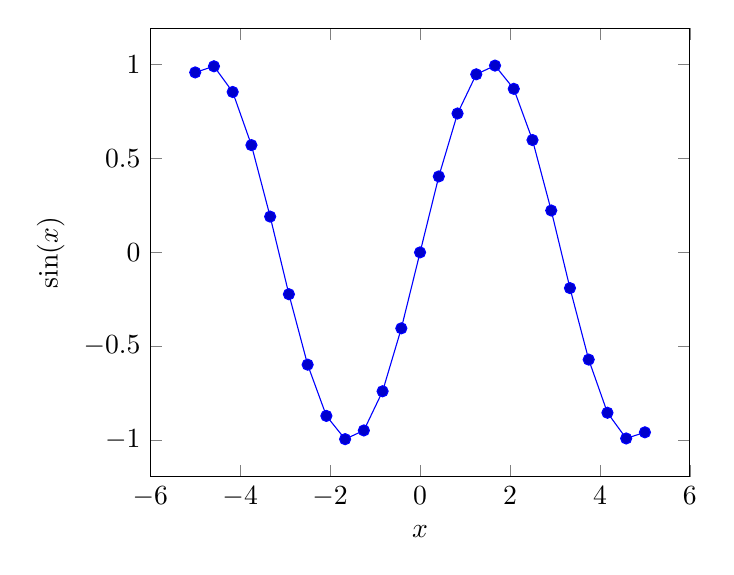
\begin{tikzpicture}
        \begin{axis}[xlabel=$x$,
            ylabel=$\sin(x)$]
          \addplot {sin(deg(x))};  % Print sine function
        \end{axis}
      \end{tikzpicture}
    \end{center}
    \caption{Plot of $\sin(x)$ direclty inside the figure environment with pgfplots.}
  \end{figure}

  \begin{figure}[h]
    \begin{center}
      \begin{tikzpicture}
        \begin{axis}[xlabel=$x$,
            ylabel=$y$]
          \addplot table [x=a, y=c, col sep=comma] {data/data.csv};  % Read coordinates from csv file and plot them
        \end{axis}
      \end{tikzpicture}
    \end{center}
    \caption{Coordinates $x$ and $y$ read from csv file and plotted pgfplots.}
  \end{figure}

}{}


%%%%%%%%%%%%%%%%%%%%%%%%%%%%%%%%%%%%%%%%%%%%%%%%%%%%%%%%%%%%%%%%%%%%%%%%%%%%%%
\section{Figures with tikz}
%%%%%%%%%%%%%%%%%%%%%%%%%%%%%%%%%%%%%%%%%%%%%%%%%%%%%%%%%%%%%%%%%%%%%%%%%%%%%%
The tikz is a package for creating graphics programmatically. With this package grids or other regular strucutres can be easliy generated.

\begin{figure}[ht]
  \begin{center}
    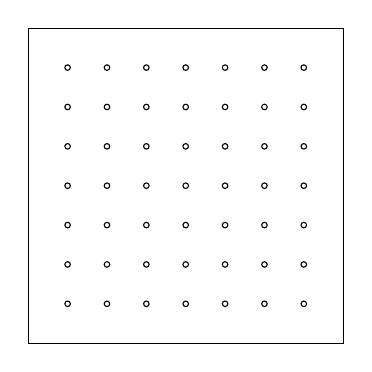
\begin{tikzpicture}
      \draw(0,0) rectangle (4,4);
      \foreach \x in {0.5,1,1.5,2,2.5,3,3.5}
      \foreach \y in {0.5,1,1.5,2,2.5,3,3.5}
      \draw(\x,\y) circle (1pt);
    \end{tikzpicture}
  \end{center}
  \caption{A regular grid genrated with easily with two for loops.}\label{fig:tikz_example}
\end{figure}


%%%%%%%%%%%%%%%%%%%%%%%%%%%%%%%%%%%%%%%%%%%%%%%%%%%%%%%%%%%%%%%%%%%%%%%%%%%%%%
\section{UML diagrams using tikz-uml}
%%%%%%%%%%%%%%%%%%%%%%%%%%%%%%%%%%%%%%%%%%%%%%%%%%%%%%%%%%%%%%%%%%%%%%%%%%%%%%

\Cref{fig:uml} presents a class diagram typeset using tikz-uml.

\begin{center}
\begin{figure}
\begin{tikzpicture}
\begin{umlpackage}{p}
\begin{umlpackage}{sp1}
\umlclass[template=T]{A}{
  n : uint \\ t : float
}{}
\umlclass[y=-3]{B}{
  d : double
}{
  \umlvirt{setB(b : B) : void} \\ getB() : B}
\end{umlpackage}
\begin{umlpackage}[x=10,y=-6]{sp2}
\umlinterface{C}{
  n : uint \\ s : string
}{}
\end{umlpackage}
\umlclass[x=2,y=-10]{D}{
  n : uint
  }{}
\end{umlpackage}

\umlassoc[geometry=-|-, arg1=tata, mult1=*, pos1=0.3, arg2=toto, mult2=1, pos2=2.9, align2=left]{C}{B}
\umlunicompo[geometry=-|, arg=titi, mult=*, pos=1.7, stereo=vector]{D}{C}
\umlimport[geometry=|-, anchors=90 and 50, name=import]{sp2}{sp1}
\umlaggreg[arg=tutu, mult=1, pos=0.8, angle1=30, angle2=60, loopsize=2cm]{D}{D}
\umlinherit[geometry=-|]{D}{B}
\umlnote[x=2.5,y=-6, width=3cm]{B}{A note with respect to class B}
\umlnote[x=7.5,y=-2]{import-2}{A anotation}
\end{tikzpicture}
\caption{Class diagram generated with tikz-uml. Example adapted from Nicolas Kielbasiewicz.}
\label{fig:uml}
\end{figure}
\end{center}

\section{UML diagrams using PlantUML}

In case \lualatex{} is used and PlantUML is installed, UML diagrams can be defined using PlantUML.

% Only works if "--shell-escape" is activated. Please activate only if you are sure, your compilation settings are correct
%\IfFileExists{plantuml.sty}{\input{latexhints-english-plantuml}}{}


%%%%%%%%%%%%%%%%%%%%%%%%%%%%%%%%%%%%%%%%%%%%%%%%%%%%%%%%%%%%%%%%%%%%%%%%%%%%%%
\section{Linguistic Forests}
%%%%%%%%%%%%%%%%%%%%%%%%%%%%%%%%%%%%%%%%%%%%%%%%%%%%%%%%%%%%%%%%%%%%%%%%%%%%%%

\begin{filecontents*}{\democodefile}
\begin{forest}
  [VP
    [DP]
    [V’
      [V]
      [DP]
    ]
  ]
\end{forest}
\end{filecontents*}
\PrintDemo{style=parallel}


%%%%%%%%%%%%%%%%%%%%%%%%%%%%%%%%%%%%%%%%%%%%%%%%%%%%%%%%%%%%%%%%%%%%%%%%%%%%%%
\section{Tables}
%%%%%%%%%%%%%%%%%%%%%%%%%%%%%%%%%%%%%%%%%%%%%%%%%%%%%%%%%%%%%%%%%%%%%%%%%%%%%%
\cref{tab:Ergebnisse} shows results and \cref{tab:Werte} shows how numerical data can be represented in a table.
\begin{table}
  \centering
  \begin{tabular}{ccc}
    \toprule
    \multicolumn{2}{c}{\textbf{summed}} & \textbf{Title}                                                          \\ \midrule
    Table                                      & as                                                           & in      \\
    \url{tabsatz.pdf}                            & recommended                                                     & gesetzt \\

    \multirow{2}{*}{Example}                    & \multicolumn{2}{c}{a nice example}                                \\
                                                 & \multicolumn{2}{c}{for using \qq{multirow}}           \\
    \bottomrule
  \end{tabular}
  \caption[Example Table]{Exampe Table -- see \url{http://www.ctan.org/tex-archive/info/german/tabsatz/}}
  \label{tab:Ergebnisse}
\end{table}

\begin{table}
  \centering
  \begin{tabular}{l *{8}{d{3.2}}}
    \toprule

                         & \multicolumn{2}{c}{\textbf{Parameter 1}} & \multicolumn{2}{c}{\textbf{Parameter 2}} & \multicolumn{2}{c}{\textbf{Parameter 3}} & \multicolumn{2}{c}{\textbf{Parameter 4}}                                                                                                                                       \\
    \cmidrule(r){2-3}\cmidrule(lr){4-5}\cmidrule(lr){6-7}\cmidrule(l){8-9}

    \textbf{Bedingungen} & \multicolumn{1}{c}{\textbf{M}}           & \multicolumn{1}{c}{\textbf{SD}}          & \multicolumn{1}{c}{\textbf{M}}           & \multicolumn{1}{c}{\textbf{SD}}          & \multicolumn{1}{c}{\textbf{M}} & \multicolumn{1}{c}{\textbf{SD}} & \multicolumn{1}{c}{\textbf{M}} & \multicolumn{1}{c}{\textbf{SD}} \\
    \midrule

    W                    & 1.1                                      & 5.55                                     & 6.66                                     & .01                                      &                                &                                 &                                &                                 \\
    X                    & 22.22                                    & 0.0                                      & 77.5                                     & .1                                       &                                &                                 &                                &                                 \\
    Y                    & 333.3                                    & .1                                       & 11.11                                    & .05                                      &                                &                                 &                                &                                 \\
    Z                    & 4444.44                                  & 77.77                                    & 14.06                                    & .3                                       &                                &                                 &                                &                                 \\
    \bottomrule
  \end{tabular}

  \caption{Example table for 4 constraints (W-Z), each having 4 parameters with (M und SD). Note: use always the same number of decimal places.}
  \label{tab:Werte}
\end{table}

\IfFileExists{pgfplotstable.sty}{

\subsection{Tables with pgfplots}
With the pgfplotstable package tables can be directly generated from a csv file.

\begin{table}[h]
\centering
\pgfplotstabletypeset[
col sep = comma,
every head row/.style={before row=\toprule,after row=\midrule},
every last row/.style={after row=\bottomrule},
display columns/0/.style={string type,column name={}}
]
{data/data.csv}
\caption{Table direclty generated from the values of a csf file.}
\end{table}
}{}


\section{Tables spanning multiple pages}


\begin{longtable}{|l|l|l|}
\caption{A sample long table.} \label{tab:long} \\

\hline \multicolumn{1}{|c|}{\textbf{First column}} & \multicolumn{1}{c|}{\textbf{Second column}} & \multicolumn{1}{c|}{\textbf{Third column}} \\ \hline
\endfirsthead

\multicolumn{3}{c}%
{{\bfseries \tablename\ \thetable{} -- continued from previous page}} \\
\hline \multicolumn{1}{|c|}{\textbf{First column}} & \multicolumn{1}{c|}{\textbf{Second column}} & \multicolumn{1}{c|}{\textbf{Third column}} \\ \hline
\endhead

\hline \multicolumn{3}{|r|}{{Continued on next page}} \\ \hline
\endfoot

\hline \hline
\endlastfoot

A & BC & D \\
A & BC & D \\
A & BC & D \\
A & BC & D \\
A & BC & D \\
A & BC & D \\
A & BC & D \\
A & BC & D \\
A & BC & D \\
A & BC & D \\
A & BC & D \\
A & BC & D \\
A & BC & D \\
A & BC & D \\
A & BC & D \\
A & BC & D \\
A & BC & D \\
A & BC & D \\
A & BC & D \\
A & BC & D \\
A & BC & D \\
A & BC & D \\
A & BC & D \\
A & BC & D \\
A & BC & D \\
A & BC & D \\
A & BC & D \\
A & BC & D \\
A & BC & D \\
A & BC & D \\
A & BC & D \\
A & BC & D \\
A & BC & D \\
A & BC & D \\
A & BC & D \\
A & BC & D \\
A & BC & D \\
A & BC & D \\
A & BC & D \\
A & BC & D \\
A & BC & D \\
A & BC & D \\
A & BC & D \\
A & BC & D \\
A & BC & D \\
A & BC & D \\
A & BC & D \\
A & BC & D \\
A & BC & D \\
A & BC & D \\
A & BC & D \\
A & BC & D \\
A & BC & D \\
A & BC & D \\
A & BC & D \\
A & BC & D \\
A & BC & D \\
A & BC & D \\
A & BC & D \\
A & BC & D \\
A & BC & D \\
A & BC & D \\
A & BC & D \\
A & BC & D \\
A & BC & D \\
A & BC & D \\
A & BC & D \\
A & BC & D \\
A & BC & D \\
A & BC & D \\
A & BC & D \\
A & BC & D \\
A & BC & D \\
A & BC & D \\
A & BC & D \\
A & BC & D \\
A & BC & D \\
A & BC & D \\
A & BC & D \\
A & BC & D \\
\end{longtable}


%%%%%%%%%%%%%%%%%%%%%%%%%%%%%%%%%%%%%%%%%%%%%%%%%%%%%%%%%%%%%%%%%%%%%%%%%%%%%%
\section{Abbreviations}
%%%%%%%%%%%%%%%%%%%%%%%%%%%%%%%%%%%%%%%%%%%%%%%%%%%%%%%%%%%%%%%%%%%%%%%%%%%%%%
At the first pass the \gls{fr} was 5.
At the second pass was \gls{fr} 3.
The plural form can be seen here: \glspl{er}.
To demonstrate what the list of abbreviations looks like for longer description texts, \glspl{rdbms} must be mentioned here.

With \verb+\gls{...}+ you can enter abbreviations, the first time you call it, the long form is used.
When reusing \verb+\gls{..}+ the short form is automatically displayed.
The abbreviation is also automatically inserted in the abbreviation list.
With \verb+\glspl{...}+ the plural form is used.
If you want the short form to appear directly at the first use, you can use \verb+\glsunset{..}+ to mark an abbreviation as already used.
The opposite is achieved with \verb+\glsreset{..}+.

Abbreviations are defined in \verb+\content\ausarbeitung.tex+ by means of \verb+\newacronym{...}{...}{...}+.

More information at: \url{http://tug.ctan.org/macros/latex/contrib/glossaries/glossariesbegin.pdf}
%%%%%%%%%%%%%%%%%%%%%%%%%%%%%%%%%%%%%%%%%%%%%%%%%%%%%%%%%%%%%%%%%%%%%%%%%%%%%%
\section{References}
%%%%%%%%%%%%%%%%%%%%%%%%%%%%%%%%%%%%%%%%%%%%%%%%%%%%%%%%%%%%%%%%%%%%%%%%%%%%%%
For distant sections \qq{varioref} is recommended:
\qq{See \vref{sec:mf}}.
The command \texttt{\textbackslash{}vref} works similar to \texttt{\textbackslash{}cref} the difference beeing that a reference to the page is additionally added.
\texttt{vref}: \qq{\vref{sec:firstsectioninlatexhints}}, \texttt{cref}: \qq{\cref{sec:firstsectioninlatexhints}}, \texttt{ref}: \qq{\ref{sec:firstsectioninlatexhints}}.

If \qq{varioref} causes difficulties, then \qq{cref} can be used instead.
This also creates the word \qq{section} automatically: \cref{sec:mf}.
This is also possible for illustrations etc.
In English please use \verb1\Cref{...}1 (with large \qq{C} at the beginning).

%With MiKTeX installation from 2012-01-16 no longer necessary.
%If a section becomes longer than one page and you want to refer to a specific place in the section with \texttt{\textbackslash{}vref}, then you should use \texttt{\textbackslash{}phantomsection} then using \texttt{vref} will also display the correct page number.

%%The link location will be placed on the line below.
%%Tipp von http://en.wikibooks.org/wiki/LaTeX/Labels_and_Cross-referencing#The_hyperref_package_and_.5Cphantomsection
%\phantomsection
%\label{alabel}
%View the example for \texttt{\textbackslash{}phantomsection} in the \LaTeX{} source code.

%Here is the example: See Section \vref{hack1} and Section \vref{hack2}.
%%%%%%%%%%%%%%%%%%%%%%%%%%%%%%%%%%%%%%%%%%%%%%%%%%%%%%%%%%%%%%%%%%%%%%%%%%%%%%
\section{Definitions}
%%%%%%%%%%%%%%%%%%%%%%%%%%%%%%%%%%%%%%%%%%%%%%%%%%%%%%%%%%%%%%%%%%%%%%%%%%%%%%
\begin{definition}[Title]
  \label{def:def1}
  Definition Text
\end{definition}

\Cref{def:def1} shows \ldots

%%%%%%%%%%%%%%%%%%%%%%%%%%%%%%%%%%%%%%%%%%%%%%%%%%%%%%%%%%%%%%%%%%%%%%%%%%%%%%
\section{Footnotes}
%%%%%%%%%%%%%%%%%%%%%%%%%%%%%%%%%%%%%%%%%%%%%%%%%%%%%%%%%%%%%%%%%%%%%%%%%%%%%%
Footnotes are provided by the command \verb+\footnote{...}+\footnote{\label{fussnote}Example footnote.}. Citing footnotes is possible by provinding a label\verb+\footnote{\label{...}...}+ and cite the footnote with \verb+\cref{...}+ in the text\cref{fussnote}.
%%%%%%%%%%%%%%%%%%%%%%%%%%%%%%%%%%%%%%%%%%%%%%%%%%%%%%%%%%%%%%%%%%%%%%%%%%%%%%

%%%%%%%%%%%%%%%%%%%%%%%%%%%%%%%%%%%%%%%%%%%%%%%%%%%%%%%%%%%%%%%%%%%%%%%%%%%%%%
\section{Various Things}
%%%%%%%%%%%%%%%%%%%%%%%%%%%%%%%%%%%%%%%%%%%%%%%%%%%%%%%%%%%%%%%%%%%%%%%%%%%%%%
\label{sec:diff}
\ifdeutsch
  Numbers (123\,654\,789) are nicely set.
  Either in a line or as non-lining figure.
  The latter is reached by parameter \texttt{osf} at package \texttt{libertine} or.\ \texttt{mathpazo} in \text{fonts.tex}.
\fi

\begin{filecontents*}{\democodefile}
\begin{compactenum}[I.]
  \item You can also keep the numbering compact thanks to paralist
  \item and switch to a different numbering
\end{compactenum}
\end{filecontents*}
\PrintDemo{style=parallel}

The words \qq{workflow} and \qq{dwarflike} can be copied from the PDF and pasted to a text file.

\begin{filecontents*}{\democodefile}
In case \LuaLaTeX{} is used as compiler, there is no ligature at \qq{f\/l} in the word \qq{dwarflike} (in contrast to \qq{fl} at \qq{workflow}).
In other words: \qq{dwarflike} and \qq{dwarf\/like} look the same in the PDF.
In case they do not, there is an issue with Lua\LaTeX{} and the selnolig package.
\end{filecontents*}
\PrintDemo{style=parallel}
% Meta comment: The precise form of the optimal ligation suppression command may vary depending on the character pairs involved - see https://tex.stackexchange.com/q/28437/9075


%%%%%%%%%%%%%%%%%%%%%%%%%%%%%%%%%%%%%%%%%%%%%%%%%%%%%%%%%%%%%%%%%%%%%%%%%%%%%%
\section{Closing remarks}
%%%%%%%%%%%%%%%%%%%%%%%%%%%%%%%%%%%%%%%%%%%%%%%%%%%%%%%%%%%%%%%%%%%%%%%%%%%%%%
Please feel free to provide enhancements for this template and create a new ticket on GitHub (\url{https://github.com/latextemplates/uni-stuttgart-computer-science-template/issues}).


\pagestyle{empty}
\renewcommand*{\chapterpagestyle}{empty}





\chapter{Needs to be relocated}


\section{Things to read(temp list)}

https://www.microsoft.com/en-us/research/wp-content/uploads/2016/02/tr-95-51.pdf

https://docs.microsoft.com/en-us/azure/service-fabric/service-fabric-reliable-services-reliable-collections




\section{Jepsen}

\end{document}
